\documentclass[10pt]{article}
\usepackage[letterpaper,margin=0.55in]{geometry}
\usepackage[T1]{fontenc}
\usepackage{lmodern,amsmath,graphicx,microtype}
\usepackage[hidelinks]{hyperref}
\pagestyle{empty}
\setlength{\parindent}{0pt}
\setlength{\parskip}{3pt}
\newcommand{\head}[1]{\vspace{3pt}\textbf{#1}\quad}
\begin{document}
\begin{center}
{\large\bfseries Pretrained Features for Math-Step Monitoring: Input and Transfer}\\[3pt]
{\small CSI 436/536, Project P, Midterm \quad October 20, 2026\\
Jiayu Liao, Zeyu Pan, Yuhan Sun}
\end{center}
\vspace{-6pt}
\head{Question and task.}
Do frozen pretrained text features improve a standard classifier, especially with limited labels?
We classify the correctness of one math solution step using logistic regression (LR) or linear SVM.
The feature alternatives are word/character TF-IDF, MiniLM-L6-v2, and BGE-base/large-en-v1.5.
We measure $\Delta=\mathrm{AUROC}(\mathrm{embedding})-\mathrm{AUROC}(\mathrm{baseline})$.
The baseline and input construction always accompany a comparison.

\head{Data and protocol.}
Our prepared PRM800K contains 911,867 human-labeled steps (27.9\% incorrect).
Splitting by problem gives 632,422 train / 88,872 reserved validation / 190,573 test steps.
We select $C\in\{0.1,1,10\}$ by grouped CV within train. Encoders remain frozen.
The original-input learning curve uses $n\in\{20,50,100,500,2000\}$ with ten stratified training subsamples each.
Full-data and input-ablation results use one fit per condition (seed 0).
AUROC is primary here, with balanced accuracy recorded as a secondary metric.

\vspace{1pt}
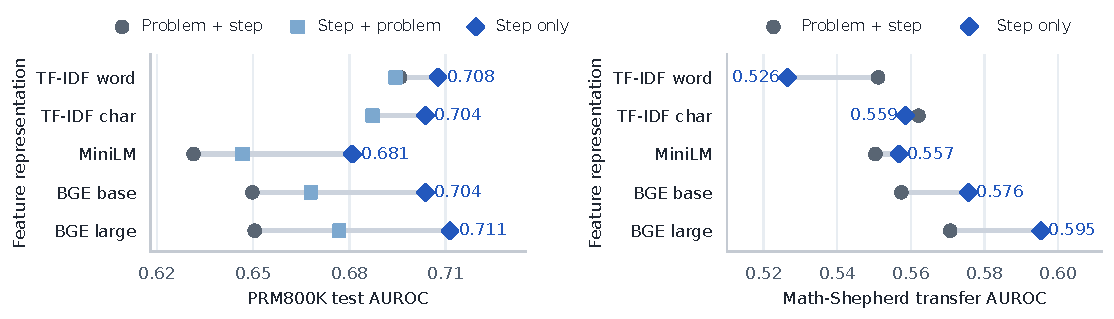
\includegraphics[width=\linewidth]{figures/one-pager-results.pdf}
\vspace{-2pt}
\begin{minipage}{\linewidth}\footnotesize
\textbf{Figure 1.} Full-training linear SVM point estimates (higher is better).
Left: changing the text supplied to the same feature family.
Right: train on PRM800K/MATH, evaluate on Math-Shepherd/GSM8K (613,666 automatically labeled steps).
Blue diamonds show step-only input. No uncertainty intervals are implied.
\end{minipage}\par

\head{Current progress.}
\textbf{Limited data:} with problem+step input, all mean AUROCs are near 0.51 at $n=20$.
For $n=50$--2000, each embedding's mean is below word TF-IDF. Seed-level differences vary in sign at small $n$.
This provides no observed sample-efficiency advantage under the original input, while step-only learning curves remain pending.
\textbf{Input ablation:} removing the problem improves embedding AUROC by 0.050--0.061, versus 0.012--0.016 for TF-IDF.
BGE-large reaches 0.711 versus word TF-IDF's 0.708 ($\Delta=+0.0038$), a point estimate rather than evidence of superiority or equivalence.
Only 0.04\% of BGE inputs truncate. This makes truncation alone an unlikely explanation, but pooling dilution remains a hypothesis.
\textbf{Transfer:} with step-only input, BGE-large reaches 0.595 versus word TF-IDF's 0.526 and char TF-IDF's 0.559.
Its gap is +0.069 versus word and +0.037 versus char. BGE-base also exceeds both baselines, whereas MiniLM (0.557) does not exceed char TF-IDF.
\textbf{Perturbations:} original-input rule-based edits change AUROC by at most 0.007 across the tested models. This does not establish general robustness or step-only robustness.

\head{Challenges and next steps.}
We corrected an early label-selection bug and reran the experiments reported here.
The input ablation is exploratory, with repeated use of the same evaluation sets.
Current TF-IDF vocabulary/IDF fitting precedes inner CV, so its tuning estimates need a fold-wise preprocessing rerun.
Existing paired bootstrap intervals resample steps, ignoring within-problem dependence, so we omit significance claims.
Next we will fix fold-wise preprocessing, compute paired problem-level intervals, and run step-only learning curves.
Separately encoding problem and step can test the dilution hypothesis.
Transfer changes task domain, data source, and labeling together, so causal attribution needs controlled follow-up.

\head{Takeaway.}
The observed benefit depends on input construction and baseline choice.
The clearest gain is BGE transfer in this tested setting, with modest absolute AUROC and confirmatory evaluation still needed.

\vspace{3pt}
{\footnotesize\textbf{Resources.}
\href{https://github.com/openai/prm800k}{PRM800K (OpenAI)},
\href{https://huggingface.co/datasets/peiyi9979/Math-Shepherd}{Math-Shepherd},
\href{https://huggingface.co/sentence-transformers/all-MiniLM-L6-v2}{MiniLM},
\href{https://huggingface.co/BAAI/bge-base-en-v1.5}{BGE-base},
\href{https://huggingface.co/BAAI/bge-large-en-v1.5}{BGE-large}.
\textbf{AI disclosure (syllabus \S4.8).}
AI assistants generated implementation code under group direction and assisted with analysis checking, figures, and rewriting these materials.
The group designed the study and data checks. Group members are responsible for understanding and verifying all submitted content.}
\end{document}
